\begin{refsection}
\chapter{Boosting in Machine Learning}

\begin{summary}
Boosting is a type of ensemble learning that combines weak learners to produce a powerful committee of prediction models. From this view, it resembles bagging, which averages the output of many, hopefully, uncorrelated models to reduce the variance. Bagging, however, is fundamentally different and instead employs forward staging additive modeling, where the data feed into a modeling procedure at the selected stage depends on the output of a growing ensemble developed in preceding stages. We start with examining AdaBoost.M1, show that it minimizes exponential loss, and extend the concept to other loss functions, both for regression and classification.
\end{summary}

Somehow surprisingly, boosting, an approach to construct and use an ensemble of predictive models, is easy to implement, is very powerful, and should be in anybody's toolbox when predictive accuracy is at stake. Similar, to bagging and random forests, boosting also relies on combination of weak learners and implements ensemble learning. But while in bagging we construct learners in parallel from sampled data, we construct boosting ensemble from data that is re-weighted according to the performance of the previously inferred learners in the sequence (Fig.~\ref{fig:bagging-vs-boosting}). In this chapter, we start with intuitive building blocks of boosted prediction models, and then dive into some of the related formalism.

\begin{figure}
\centering{
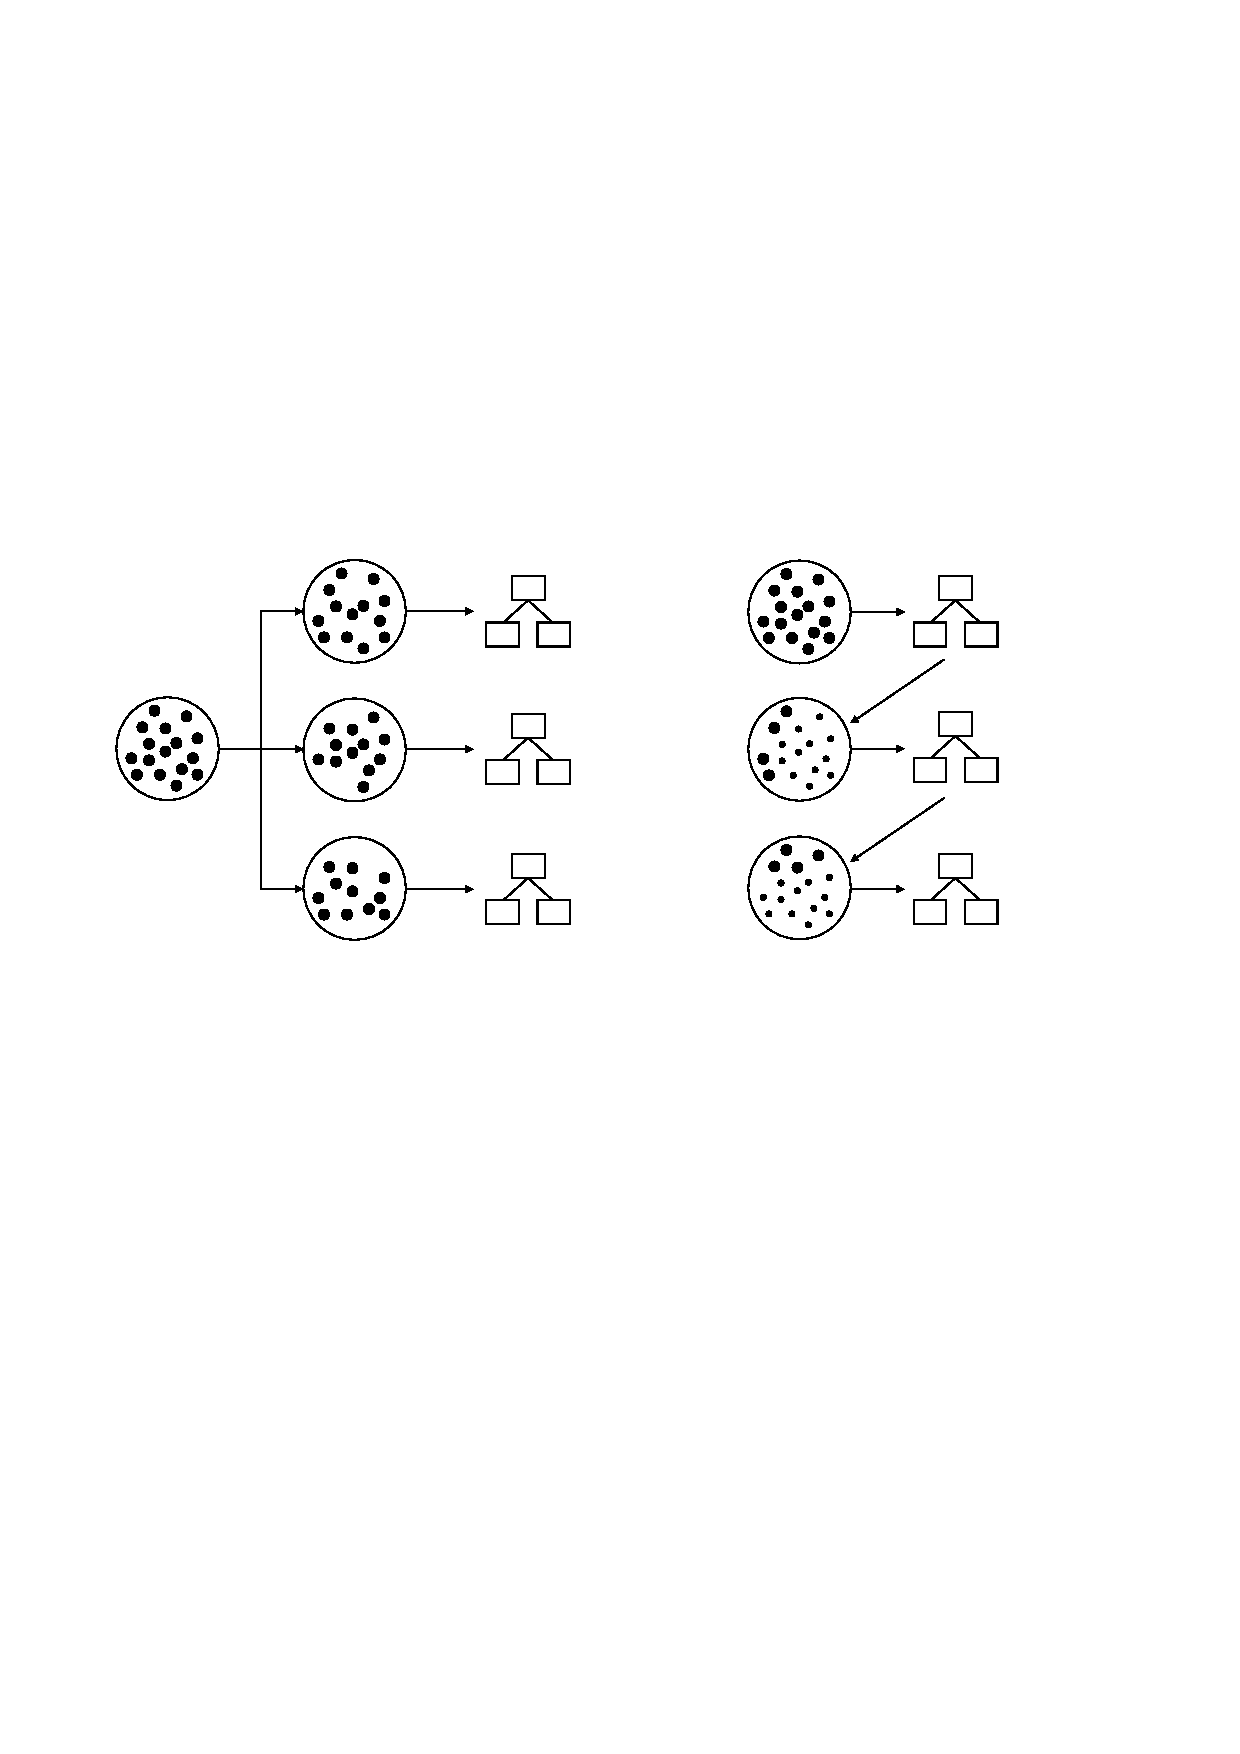
\includegraphics[width=0.8\linewidth]{figures/bagging-vs-boosting.pdf}
}
\\
\hspace{2.5cm} bagging - parallel \hspace{3cm} boosting - sequential \\
\caption{Bagging improves accuracy through ``wisdom of the crowd'', while boosting develops a sequence of models where each model specializes in prediction in the area where previous models in the sequence have failed.}
\label{fig:bagging-vs-boosting}
\end{figure}

\section{AdaBoost In a Nutshell}

Let us quickly skim through some of the concepts that are important in boosting machine learning. We use boosting both in regression and classification, and in fact, we can adapt it for any kind of supervised machine learning tasks. In this section, though, we assume we will use it for classification, and will further -- to simplify the introduction -- constrain the task to binary classification with equal class distribution.

\subsection*{Weak vs. Strong Classifiers}

Consider an error rate, $\epsilon\in[0.0,1.0]$ of a binary classifier with $y\in\{-1,1\}$ for a problem with an equal class distribution. A weak learner would produce a weak classifier that would perform only slightly better than a random classifier. That is, for an assumed problem, its error on the training set would be just slightly below $0.5$. On the other hand, in practice, we would like to develop strong classifiers with a very low error rate. Interestingly, and as a fundation for boosting, we can form a strong classifier from a set of weak classifier.

Consider a simple case of three classifiers, and let us denote them with $h^1(x)$, $h^2(x)$, and $h^3(x)$, where $x$ is a vector that describes a data instance we would like to classify. If the three classifiers are substantially different, and they make wrong predictions in disjunct areas of the data space (Fig.~\ref{fig:boosting-three-classifiers}), we can construct a simple, strong classifier as an ensemble that would join the output of the three classifiers in the following way:
\begin{equation}
H(x) = \sign(h^1(x) + h^2(x) + h^3(x))
\end{equation}
The prediction of the classifier $H(x)$, under the assumption that the areas of erroneous prediction of each of the three classifiers do not overlap. It would be great if we could construct such classifiers, but in reality, of course, the areas where classifiers get it wrong would overlap, and hence a simple procedure for their ensembling would not necessary be beneficial.

We may try to develop classifiers that are of the type from Fig.~\ref{fig:boosting-three-classifiers}, that is, where a classifier attempts to be correct in the area where a previous classifier, or a set of previous classifiers were wrong. We will do so by changing the data. We will build the first classifier, $h^1$ on the entire data set, but then try to distort the data to exaggerate on the data space where $h^1$ makes mistakes. A simple procedure we can use is through training data instance weighting: we will increase the weight of the data instances that were misclassified by $h^1$, thus instructing a new classifier $h^2$, developed on such distorted data set, to correctly classify the data instances which were misclassified by $h^1$. If we follow the idea from the previous paragraph and try to develop three different classifiers, we now can train the third one on a data set where the weights of the data instances would emphasize those $x$ where $h^1(x)\neq h^2(x)$.

Just a quick note: thus far, our classification inference algorithm never considered data instance weights. It is not difficult to change the inference algorithm to do so. For instance, in inference of trees, instead of counts of the data instances we would sum up the weights. Where changing the training algorithms to handle weights is not possible, we could address the exaggeration with oversampling of the target data instances.

\begin{figure}
\centering{
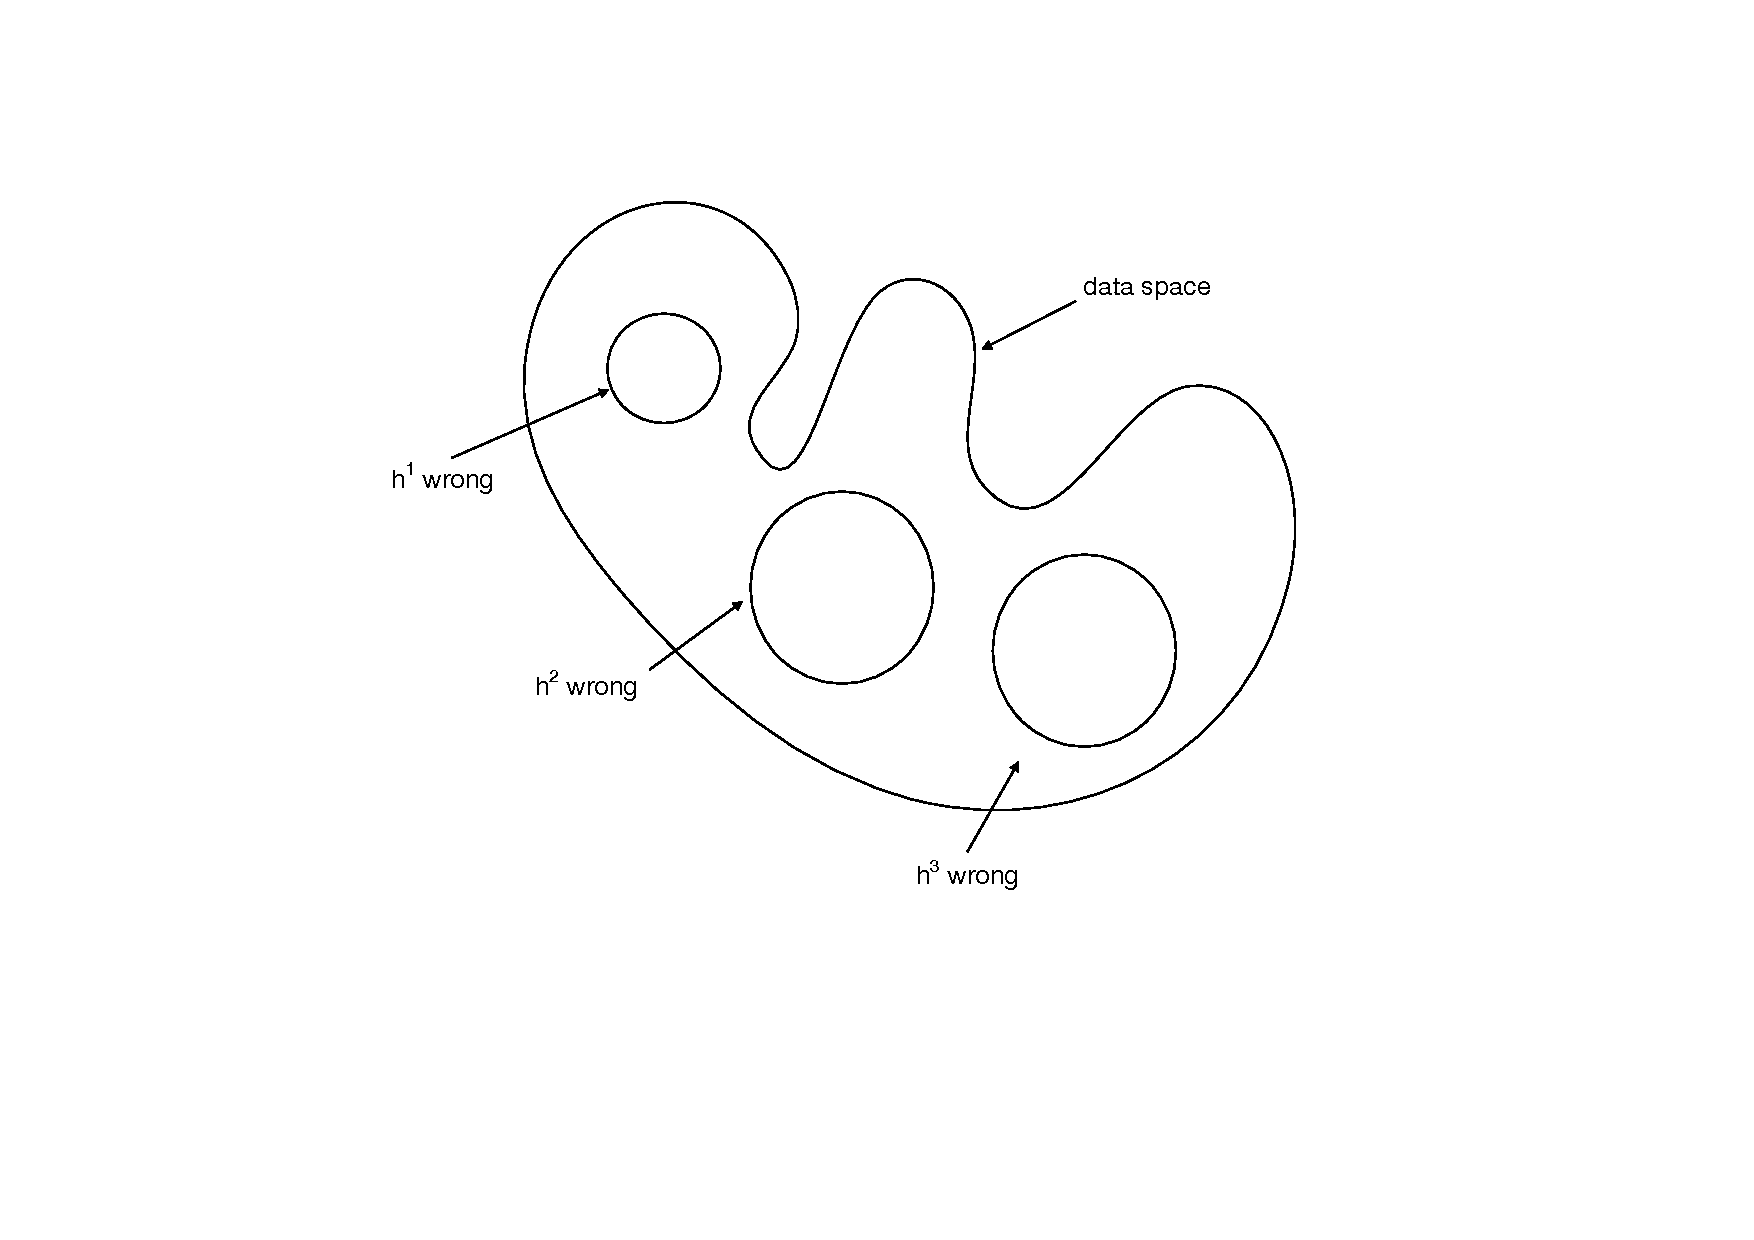
\includegraphics[width=0.5\linewidth]{figures/boosting-three-classifiers.pdf}
}
\caption{A hypothetical data space and three classifiers with disjunctive areas where their prediction is incorrect.}
\label{fig:boosting-three-classifiers}
\end{figure}

\subsection*{Hierarchy of predictors}

If constructing a classifier by ensembling the predictors works well, we could improve those predictors as well through ensembling them from another, nested set of classifiers. By doing this we would shrink the area where the predictors make mistakes, making it easier for a base set of predictors not to overlap in their misclassification zones. Note that in theory we may continue building such hierarchy to arbitrary level, whereas practically and in most cases development of one serious of predictors suffices.

\subsection*{A Weak Classifier and Initial Data Instance Weights}

We hinted about the use of weak classifiers, but have not yet introduced an algorithm to construct them. Here it is: a {\em decision tree stump}. This learning algorithm uses a decision tree inference algorithm, but limits the depth of the tree to one, that is, besides the root node there is only a next level with a set of leaves. Stumps use only one feature to decide which leave node to use for prediction. In practice, we can employ shallow trees that are deeper than one level, but for an example of a weak classifier a decision tree stumps would do as well. Also notice that while our introduction talks about classifiers, we can use trees for regression as well and hence we will also be able to develop bootstrap predictors for regression problems.

Note that we can use boosting with any kind of prediction models. But due to speed and simplicity, and since they are weak classifiers, we use shallow trees in practical implementations.

The error rate of a classifier can be expressed as:
$$\epsilon = \sum_\text{wrong}{1\over N}$$
where $N$ is the number of data instances in the training set. Initially, all instances will have equal weight and since we would like the weights to form a distribution and hence sum to $1$, the weights for each data instance $i$ for the first classifier, that is $h^1$, are:
$$w_i^1 - {1\over N}$$
Using the formulation above, we can express the error rate as a function of weights:
$$\epsilon = \sum_{\text{wrong}} w_i$$

\subsection*{Ensembling Classifiers}

A more general way to combine classifiers, rather than summing their outputs, would be to construct their weighted combination:
$$ H(x) = \sign(\alpha^1 h^1(x) + \alpha^2 h^2(x) + \ldots + \alpha^T h^T(x)) $$
where $T$ is a number of weak classifiers which we would like to ensemble. This is again different from bagging. Bagging counts on wisdom of the crowds, while here we are summing up on series of classifiers which are different in the areas of misclassification and where we will weight them according to their error. In boosting, the wisdom of the crowds becomes the wisdom of the experts that specialize in different area of the data space.

The overall procedure to construct our ensemble is then as shown in Table~\ref{t:bootstrap-algorithm}.

\begin{table}
\caption{An overall structure of a bootstrap learner}
\begin{tabbing}
xxxx \= xxxx \= xxxx \kill
$t\leftarrow 0$ \\
$w_i^t\leftarrow {1\over N}$ \\
{\bf while} $t\leq T$ \\
\> $t\leftarrow t+1$ \\
\> {\bf pick} $h^t$ that minimizes $\epsilon^t$ \\
\> {\bf pick} $\alpha^t$ \\
\> {\bf calculate} $w^{t+1}$
\end{tabbing}
\label{t:bootstrap-algorithm}
\end{table}

Suppose that we define the weights as:
$$w_i^{t+1}={w_i^t\over z} \exp\left(-\alpha^t h^t(x_i)y_i\right)$$
where $z$ is a normalizing factor so that the weights form a distribution and they sum to 1. The equation above comes from mathematical convenience, but we will show that while initially proposed for boosting, they have a more intuitive and simpler interpretation. Notice that where the prediction $h^t(x_i)$ and the true class $y_i$ agree, and assuming that the factors $\alpha$ are positive, the future weight $w_i^{t+1}$ of the instance $i$ is lowered. When prediction and the true class do not agree, the value of the future weight $w_i^{t+1}$ is raised.

We would like to minimize the error for the ensemble. It turns out that to do this~\citep{FreundSchapire1997} we need to set the weight of the classifier according to the following:
\begin{align}
\alpha^t & ={1\over 2}\ln{1-\epsilon^t \over \epsilon^t} \label{eq-freundschapire}\\
& = \ln{\sqrt{1-\epsilon^t \over \epsilon^t}}
\end{align}

If we combine this expression with the update for the data instance weights, and note that the product $h^t(x_i)y_i$ equals $1$ for correct classification and $-1$ for misclassification, than we obtain
$$w_i^{t+1} = {w_i^t \over z} \times
\begin{cases}
\sqrt{\epsilon^t \over 1-\epsilon^t }, & \text{if correct} \\
\sqrt{1-\epsilon^t \over \epsilon^t}, & \text{if wrong}.
\end{cases}
$$
The weights have to add up to 1, thus we need to set the normalization factor to
$$
z = {\epsilon^t \over 1-\epsilon^t} \sum_\text{correct} w_i^t + {1-\epsilon^t \over \epsilon^t}\sum_\text{wrong} w_i^t
$$
Notice, however, that the sum of the weights of the missclassified items is the error rate, that is, $\sum_\text{wrong} w_i^t=\epsilon^t$. Similarly, the sum of the weight over correct classifications is one minus the error rate, that is, $\sum_\text{correct} w_i^t=1-\epsilon^t$. Hence,
$$
z = 2\sqrt{\epsilon^t (1-\epsilon^t)}
$$
Combining the expression for weight update and normalization, we obtain:
$$w_i^{t+1} = {w_i^t \over 2} \times
\begin{cases}
\sqrt{1\over 1-\epsilon^t }, & \text{if correct} \\
\sqrt{1\over \epsilon^t}, & \text{if wrong}.
\end{cases}
$$
Now, if we add the weights for the correct classifications, we get
\begin{align*}
{1\over 2}{1\over 1-\epsilon^t}\sum_\text{correct} w^t & = {1\over 2}{1\over 1-\epsilon^t} (1-\epsilon^t)\\
& = {1\over 2}
\end{align*}
Similar is true for missclassifications,
\begin{align*}
{1\over 2}{1\over \epsilon^t}\sum_\text{wrong} w^t & = {1\over 2}{1\over \epsilon^t} \epsilon^t\\
& = {1\over 2}
\end{align*}

In other words, the boosting algorithm that we have described distrubutes the same amount of weights to correct and incorrect classification. If incorrect classifications will be in minority, which we hope they will, the misclassified examples will carry higher weights for the next instance of the training algorithm in the sequence. The procedure described here is called AdaBoost for adaptive boosting and was introduced in ~\citep{FreundSchapire1997}. Interestingly, while the math for Eq.\ref{eq-freundschapire} was worked out in the original publication, the interpretation with notion that the weights for both misclassification and classification sum to one half, which does in a way simplify the update as well, was not noticed at the time.

% \section{AdaBoost}

% AdaBoost, as described in the previous section, is an example of a boosting machine learning procedure that sequentially applies the weak classification algorithm to repeatedly modified version of the training data by increasing the weights of the misclassified data instances. The procedure dramatically increases the performance of weak learners, which is shown in often exponential decrease of the error rate on the test set with increasing number of classifiers in the sequence. We here explore why is this so, what loss function are we optimizing and the review other algorithms in this class.

% Let us start with the decision rule, or the output of the AdaBoost with $M$ predictors:
% \begin{equation}
% H(x)=\sign\left( \sum_{m=1}^M \alpha^m h^m(x)) \right) 
% \end{equation}


\printbibliography[heading=subbibliography]
\end{refsection}